\subsection{Komponenten}
Bei den Komponenten musste darauf geachtet werden, dass diese den äusseren Einflüssen sowie den spezifischen Softwaretechnischen Daten genügen. Die einzelnen Geräte der Arbeit bestehen aus Rechnereinheit, Messsensor, WIFI-Adapter, Gehäuse sowie einer Spannungsversorgung.

\subsubsection{Rechnereinheit}
An die Rechnereinheit wurden sehr grosse Anforderungen gestellt, da diese bei $-40^\circ\text{C}$ aber auch bei über $40^\circ\text{C}$ die Auswertung korrekt durchführen muss. Ebenso muss die Rechnereinheit sehr viel Auswertungen direkt durchführen, um so wenig wie möglich direkt zu speichern. Der Rechnerkern des Gerätes besteht aus einem Allwinner H3, welcher einen Quad-core Cortex-A7 mit bis zu 1.2 GHz Taktrate besitzt. Dieser Rechnerkern ist einer der am Besten geeignetsten für das Gerät, da auf diesem mehrere Prozesse gleichzeitig ablaufen können. Dies ist nötig um die gewünschte Verarbeitungsgeschwindigkeit zu erreichen. Im Zuge dessen wurde ein vorgefertigtes Board im Gerät eingesetzt. Das eingesetzte Board ist ein NanoPi NEO von FriendlyARM \cite{NanoPi}. Der NanoPi NEO hat den oben genannten Quad-core Prozessor, mitwelchem die Aufgabe gelöst werden kann. \\
Dieses Board bietet ebenso den Vorteil, dass sich alles auf einer Fläche von 40x40 cm  befindet. So kann das gesamte Gerät sehr kompakt gestaltet werden. Das Board wird mit einer externen Speicherkarte verwendet, auf welcher sich das Betriebssystem befindet. Im Falle von Fast and Curious ist es Ubuntu 16.04 (Long Time Supported). \\
Nachteil am NanoPi NEO sind zum einen die eher schlechte Dokumentation sowie das Vorhandensein von lediglich eines einzelnen USB Anschlusses. Aus diesem Grunde musste beim  Gerät ein USB Hub verwendet werden um den Messsensor sowie den USB-WIFI-Adapter anzuschliessen. Nachfolgendes Bild (\fref{bLayout}) zeigt das Layout des NanoPi NEO.

\begin{figure}[H]
  \centering
  \includegraphics[width=0.99\textwidth]{Hardware/NanoPi_Neo.jpg} 
  \caption{Layout des NanoPi NEO. \cite{NanoPiNeo}}
  \label{bLayout}
\end{figure}

\subsubsection{Messsensor}
Der Messsensor des Gerätes muss in der Lage sein, Daten der Verkehrsteilenehmer zu liefern, mit denen dann die weitere Auswertung geschehen kann. Es müssen aus den Daten des Messsensors Kenngrössen extrahiert werden, welche die Verkehrsteilnehmer eindeutig identifizieren lässt. Es wurde auf eine Kamera zurückgegriffen, welche im Stande ist zwei Fahrspuren zu überdecken und mindestens drei Bilder pro vorbeifahrendem Verkehrsteilnehmer aufzunehmen. \\
Mithilfe nachfolgender Berechnung wurde die geeignete Kamera sowie das passende Objektiv dazu gefunden. Die Skizze (\fref{bBerechnung}) zeigt die schematische Darstellung eines Aufstellpunktes des Geräts.
\begin{citemize}

\item Kamera mit 30 FPS \\
$l_{ 1,30 } = \frac{ 22.22 m/s }{ 30 FPS} = 0.75 m$ \\ 
$l_{ 4,30 } = 4 * l_{1,30} = 3 m$\\
$\alpha_{30} = 2* \arctan(l_{4,30 }) \approx 150^\circ$ \\\\


\item Kamera mit 60 FPS \\
$l_{ 1,60 } = \frac{ 22.22 m/s }{ 60 FPS} = 0.37 m$ \\ 
$l_{ 4,60 } = 4 * l_{1,30} \approx 1.5 m$\\
$\alpha_{60} = 2* \arctan(l_{4,60 }) \approx 120^\circ$ \\\\
\end{citemize}

\begin{figure}[H]
  \centering
  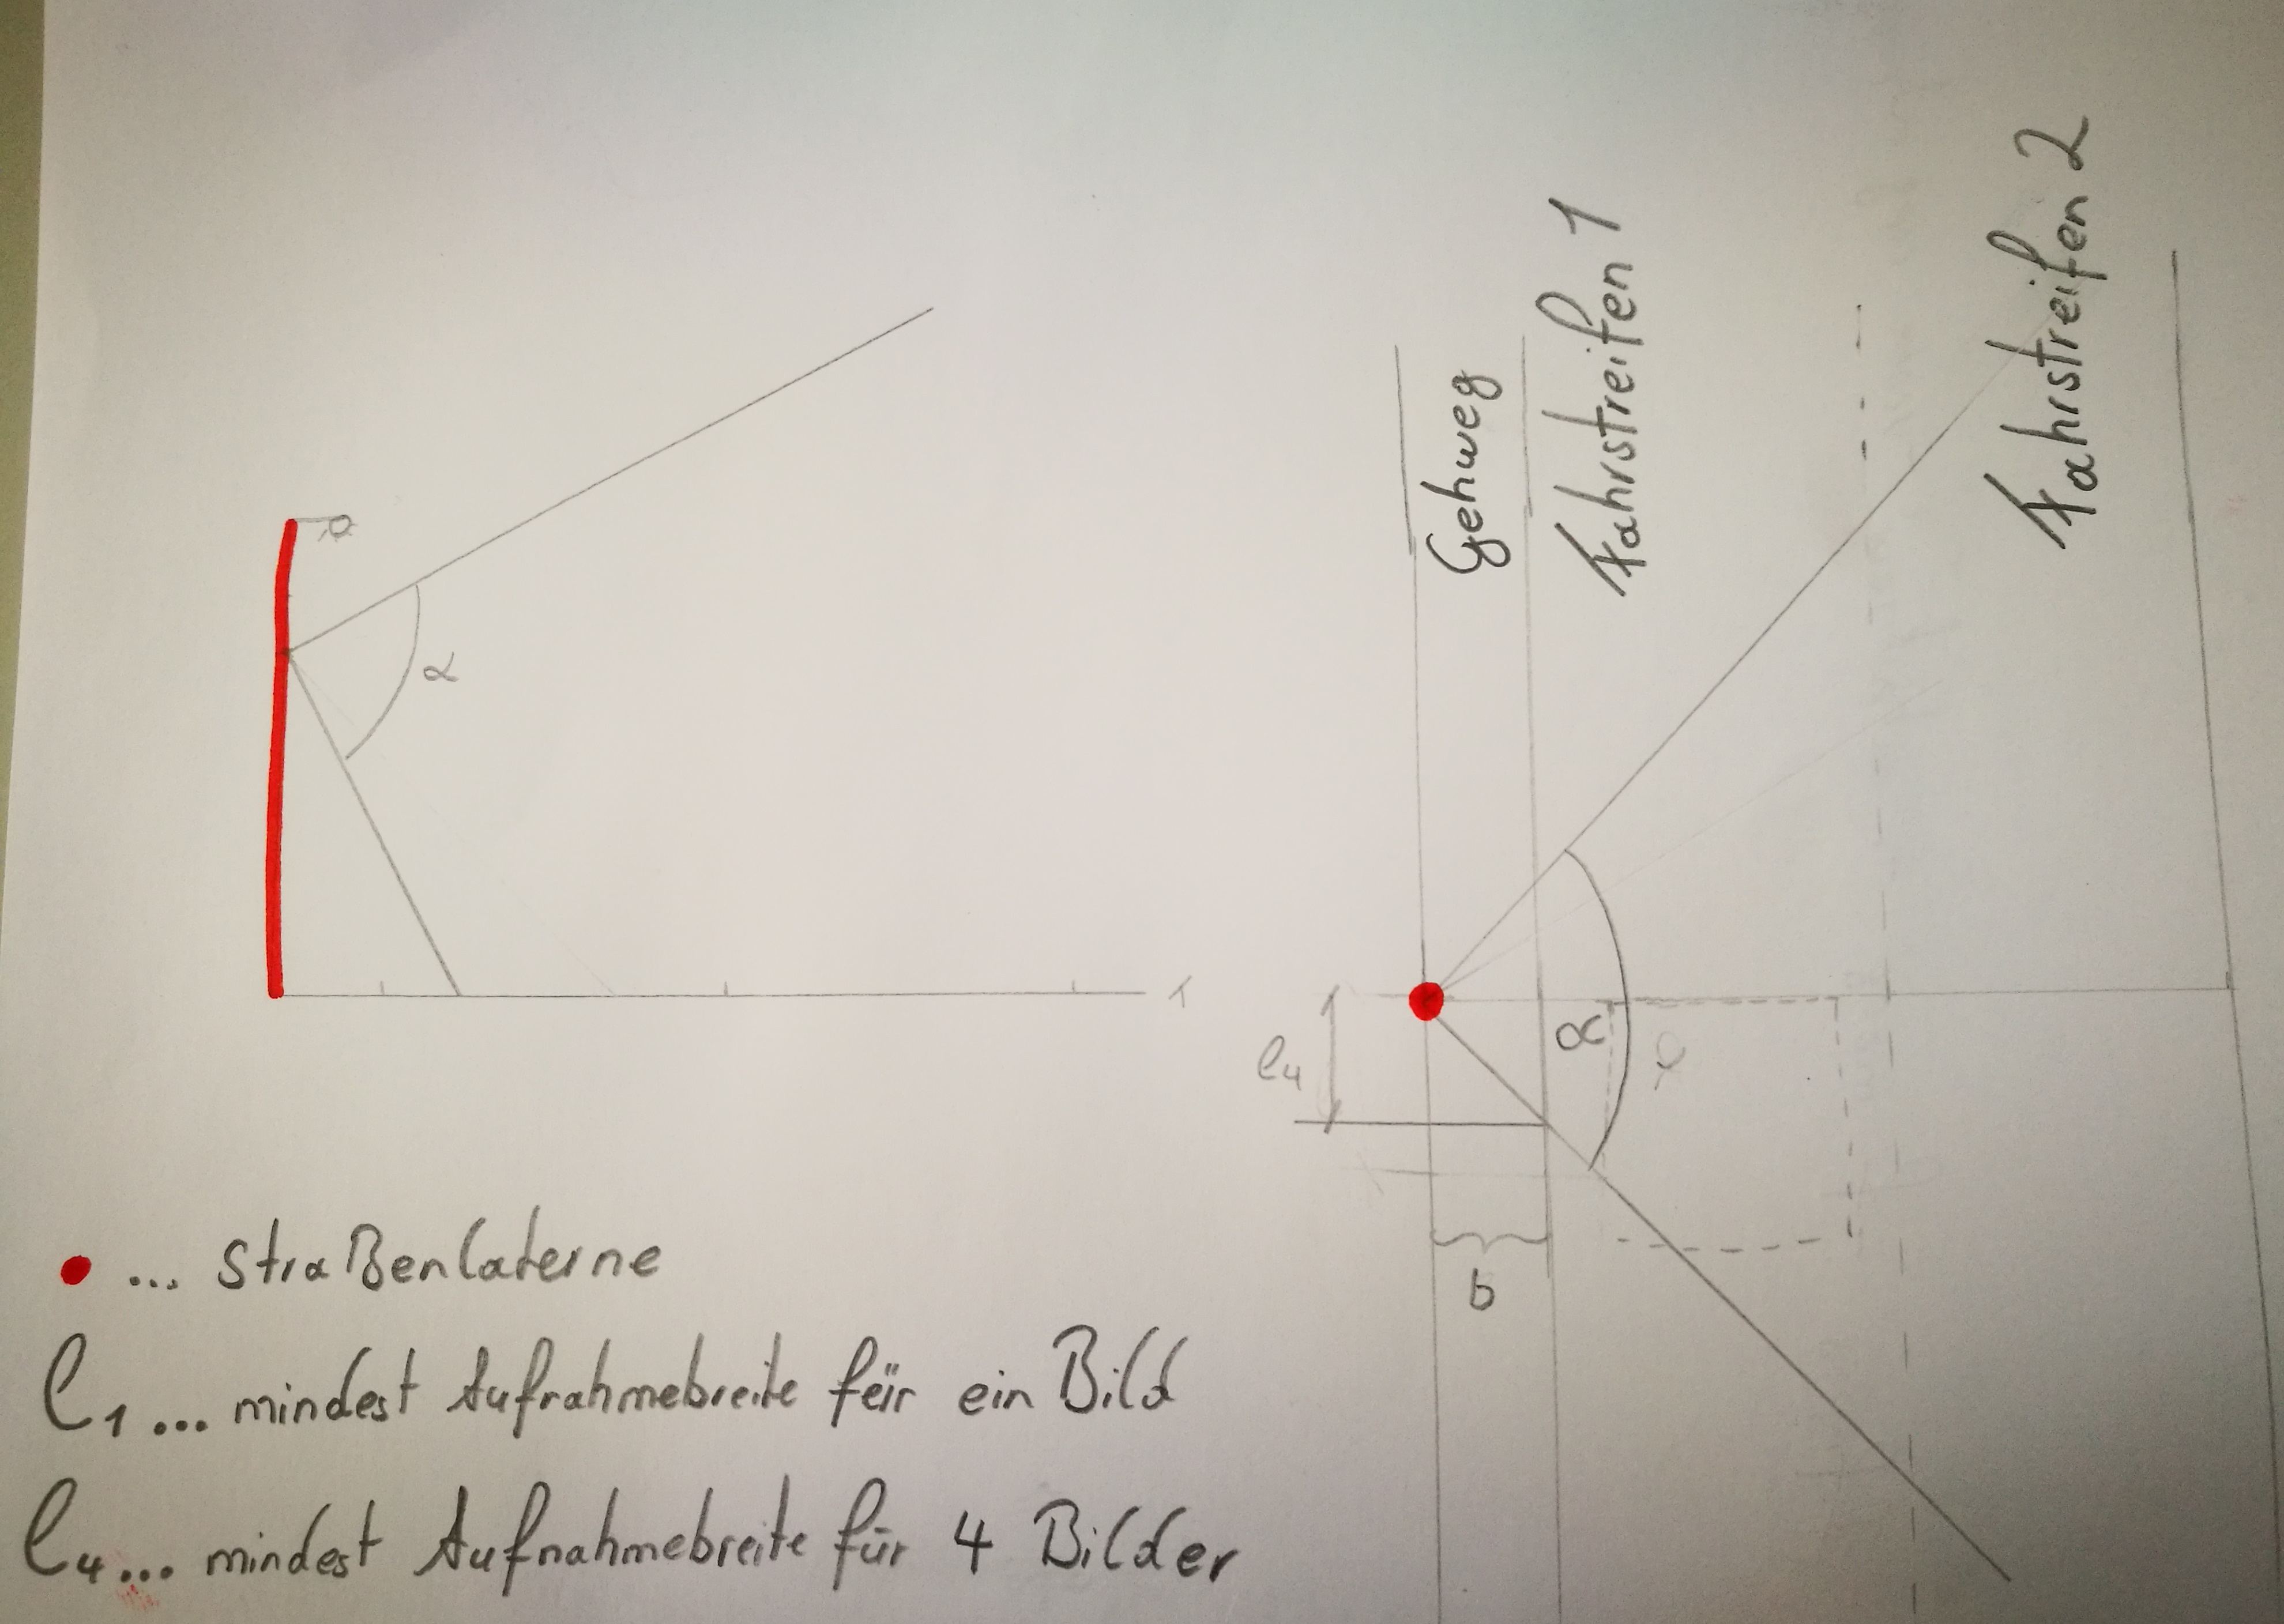
\includegraphics[height=0.49\textwidth]{Hardware/ObjektivBerechnung.jpg} 
  \caption{Skizze zur Berechnung der Kamera Daten.}
  \label{bBerechnung}
\end{figure}

Durch diese Berechnung wurde eine Kamera eingesetzt, welche mit einer Framerate von 60 FPS Bilder aufnimmt. \\
Im produzierten Prototypen wurde eine "'ELP 1080p Full HD H.264"' Kamera mit 3.6 mm Objektiv verwendet. Diese Kamera hat den Vorteil, dass die gewünschten Treiber auf dem Betriebssystem schon installiert sind und die Kamera sehr preisgünstig zu haben ist. Diese Kamera besitzt bei einer FPS Anzahl von 60 eine Auflösung von 640x480 Pixel und einem 3.6 mm Objektiv. Diese Anzahl an Pixel reicht aus, um die nötigen Daten der Verkehrsteilnehmer zu extrahieren. \cite{Kamera}

\subsubsection{WIFI-Adapter}
Um das Gerät Steuern und Überwachen zu können, wird eine kabellose Verbindung benötigt. Dies ist am einfachsten über eine WIFI-Verbindung zu erreichen. Da das NanoPi NEO keine internen Funksender eingebaut hat, wird ein WIFI-Adapter benötigt. Dazu kann jeder WIFI-Adapter verwendet werden, welche das Linux System unterstützen und somit ein Treiber vorhanden ist. Werden für die Geräte unterschiedliche WIFI-Adapter eingesetzt, so muss nach der Anleitung für die Installation der Geräte vorgegangen werden und die Namen der Adapter geändert werden.\\
Die einzige Anforderung an den WIFI-Adapter ist es, dass dieser über USB angeschlossen wird. Die Geräte, welche produziert wurden, haben unterschiedliche WIFI-Adapter eingebaut und es funktioniert mit allen WIFI-Adaptern ohne irgendwelche Probleme. Die Verbindung geschieht über einen Hotspot vom Endgerät zu NanoPi NEO.

\subsubsection{Spannungsversorgung}
Die Spannungsversorgung der Geräte wurde mittels Autobatterie und Spannungswandler realisiert. Das gesamte Gerät benötigt bei Volllast ca. 400 mA Strom. Die verwendeten Autobatterien haben eine Kapazität von 44 Ah und eine Spannung von 12 V. \\

$\frac { 44000\quad mAh\quad \times \quad 12\quad V }{ 400\quad mAh\quad \times \quad 5\quad V } =\quad 264\quad h=\quad 11 d$ \\

Wie aus dieser Berechnung entnommen werden kann, beläuft sich die Betriebszeit mit einer Akku Ladung theoretisch auf ca. 11 Tage. Wie erwartet ist die tatsächliche Laufzeit der Geräte kleiner als die Berechnete. Jedoch beträgt die tatsächliche Laufzeit etwa die Hälfte von ca. 5 Tagen. \\
In einer tatsächlichen Fertigung der Geräte muss eine neue Spannungsquelle gefunden werden, da Autobatterien beinahe immer Bleihaltig sind. Es könnten Lithium Ionen Akkus verwendet werden, jedoch waren diese für die Prototypen zu teuer und nicht rentabel. 

\subsubsection{Gehäuse}
Das Gehäuse der Prototypen besteht aus einer Kunststoffbox, in welcher sich früher Lebensmittel befanden. In diesem Gehäuse wurden alle Komponenten welche oben genannt wurden, mittels Klettverschluss angebracht, um die Komponenten ohne Gehäuse weiter zu verwenden. Dies ermöglichte eine leichtere Bedienung bei der Programmierung der Software. Am Gehäuse wurden zwei Gewindestangen angebracht, um die Ausrichtung des Gerätes einstellen zu können. Des Weiteren wurde im Deckel der Kunststoffboxen Schlitze geschnitten, um die Abwärme der Komponenten besser nach aussen zu befördern. Die Gehäuse werden an den Strassenlaternen mittels grossen Kabelbindern befestigt.\\
\textbf{Wichtig: In den Gehäusen befindet sich keine Batterie.}\\
Aus Sicherheitsgründen wurde ein zweipoliges Kabel von den Geräten nach unten gezogen und an den Polen der Batterie befestigt. Das folgende Bild (\fref{bGehäuse}) dient dabei zur Illustration des leeren Gehäuses.

\begin{figure}[H]
  \centering
  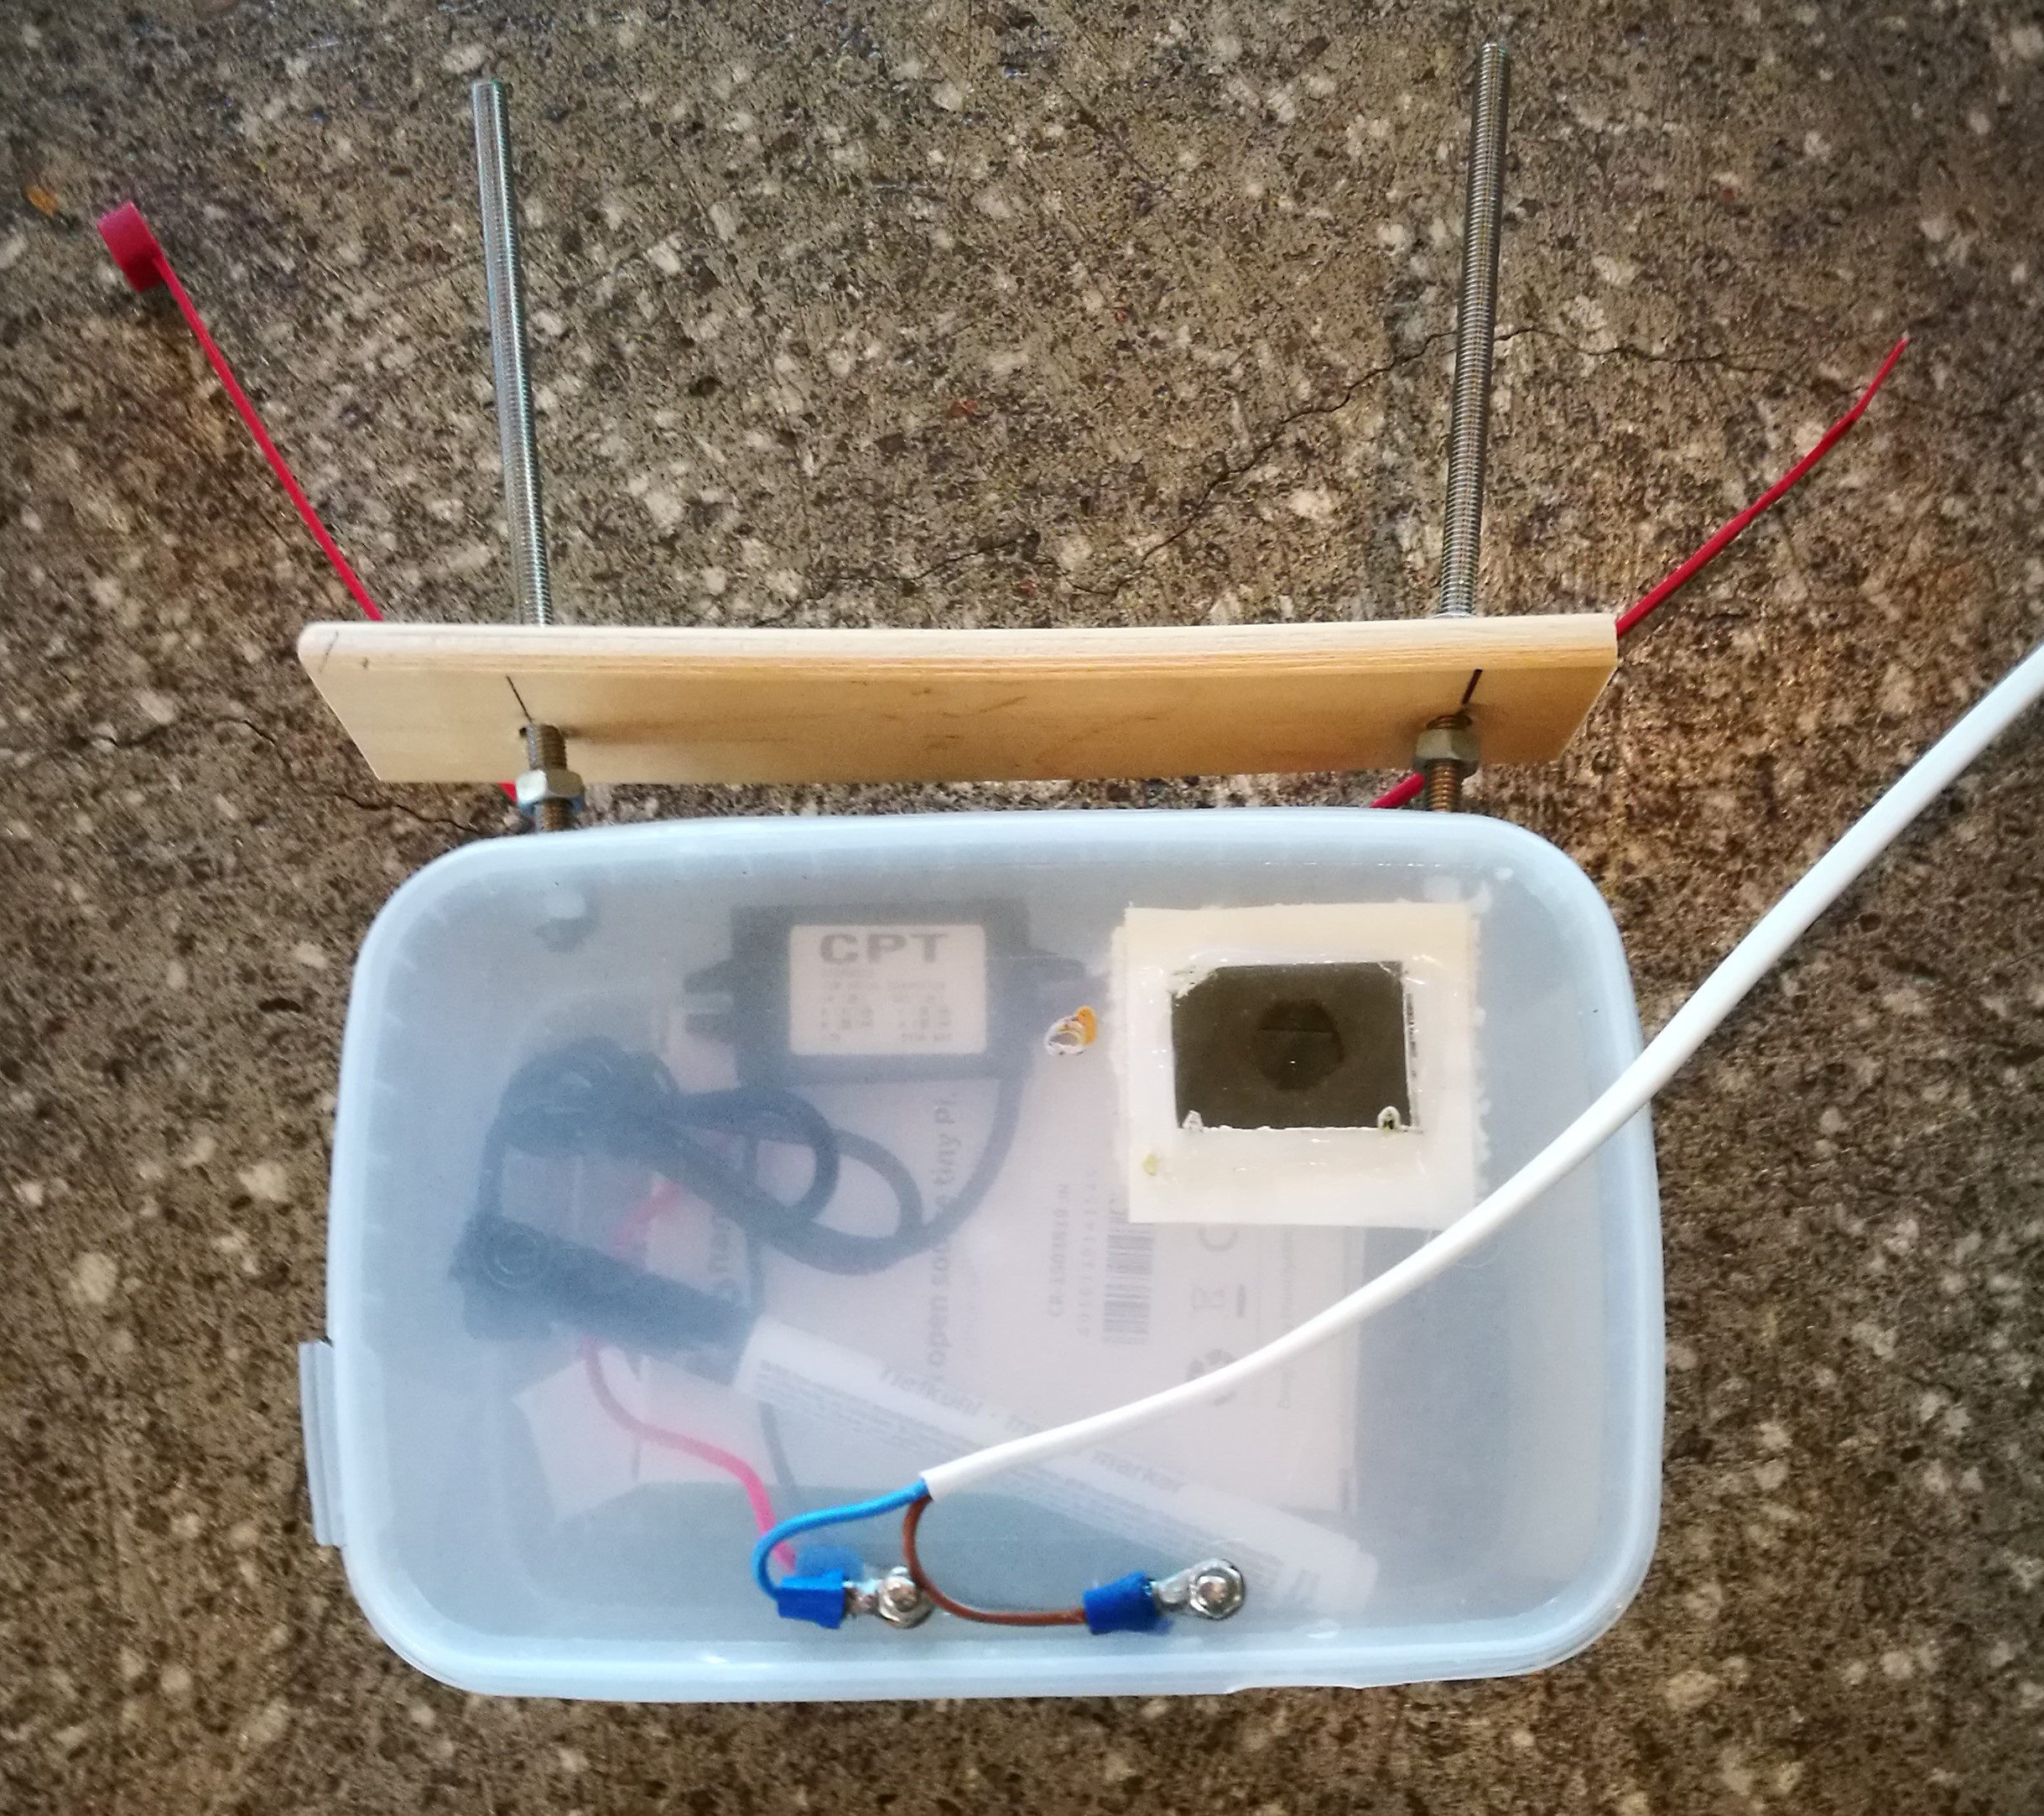
\includegraphics[height=0.49\textwidth]{Hardware/Gehaeuse.jpg} 
  \caption{Foto eines leeren Gehäuses.}
  \label{bGehäuse}
\end{figure}